%%%%%%%%%%%%%%%%%%%%%%%%%%%%%%%%%%%%%%%%%%%%%%%%%%%%%%%%%%%%%%%%%%%%%%%%%%%%%%%%
%%
%%   BornAgain User Manual
%%
%%   homepage:   http://www.bornagainproject.org
%%
%%   copyright:  Forschungszentrum Jülich GmbH 2015
%%
%%   license:    Creative Commons CC-BY-SA
%%   
%%   authors:    Scientific Computing Group at MLZ Garching
%%               C. Durniak, M. Ganeva, G. Pospelov, W. Van Herck, J. Wuttke
%%
%%%%%%%%%%%%%%%%%%%%%%%%%%%%%%%%%%%%%%%%%%%%%%%%%%%%%%%%%%%%%%%%%%%%%%%%%%%%%%%%


\newpage
\chapter{Download, installation, first steps} \SecLabel{QuickStart}

This User Manual is complementary to the online documentation
at the project web site \url{http://www.bornagainproject.org};
it does not duplicate technical information that is more conveniently
available there.
The \textsc{Download} section offers
binary packages and a source archive.
The \textsc{Documentation} section contains an overview
of the functionality,
detailed installation instructions,
tutorials and usage examples.

\begin{figure}[ht]
\begin{center}
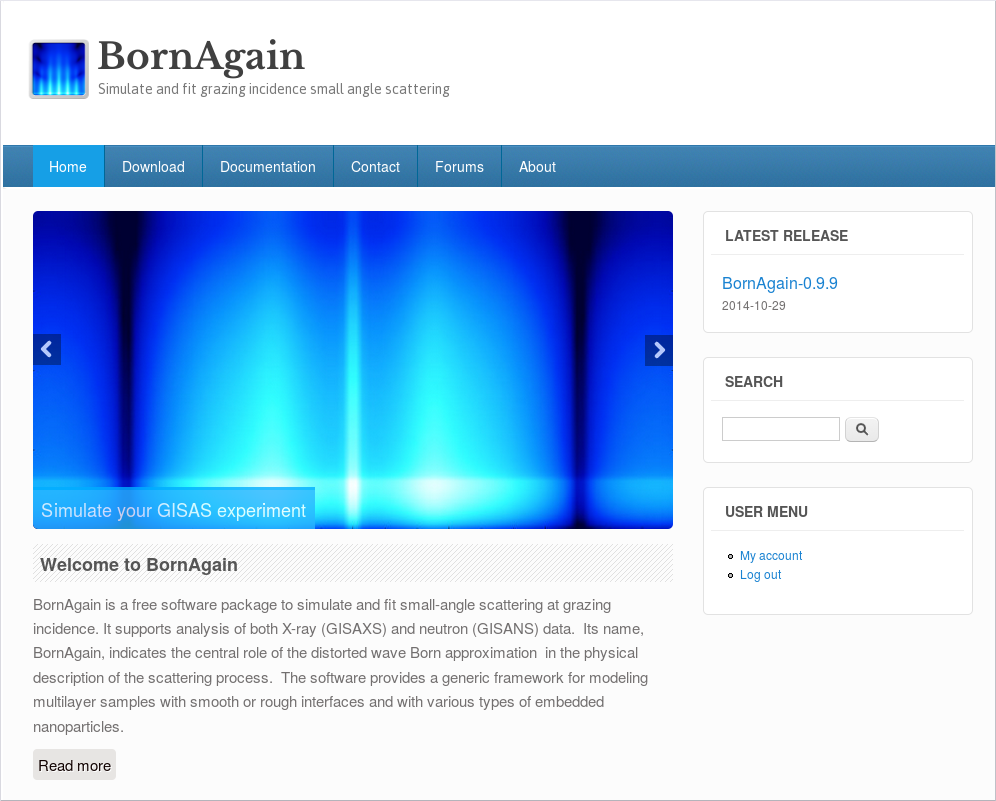
\includegraphics[width=0.83\textwidth]{Figures/screenshot/website.png}
\end{center}
\caption{A screenshot of the home page
         \url{http://www.bornagainproject.org}.}
\label{fig:website}
\end{figure}
